\documentclass[twoside]{book}

% Packages required by doxygen
\usepackage{calc}
\usepackage{doxygen}
\usepackage{graphicx}
\usepackage[utf8]{inputenc}
\usepackage{makeidx}
\usepackage{multicol}
\usepackage{multirow}
\usepackage{textcomp}
\usepackage[table]{xcolor}

% Font selection
\usepackage[T1]{fontenc}
\usepackage{mathptmx}
\usepackage[scaled=.90]{helvet}
\usepackage{courier}
\usepackage{amssymb}
\usepackage{sectsty}
\renewcommand{\familydefault}{\sfdefault}
\allsectionsfont{%
  \fontseries{bc}\selectfont%
  \color{darkgray}%
}
\renewcommand{\DoxyLabelFont}{%
  \fontseries{bc}\selectfont%
  \color{darkgray}%
}

% Page & text layout
\usepackage{geometry}
\geometry{%
  a4paper,%
  top=2.5cm,%
  bottom=2.5cm,%
  left=2.5cm,%
  right=2.5cm%
}
\tolerance=750
\hfuzz=15pt
\hbadness=750
\setlength{\emergencystretch}{15pt}
\setlength{\parindent}{0cm}
\setlength{\parskip}{0.2cm}
\makeatletter
\renewcommand{\paragraph}{%
  \@startsection{paragraph}{4}{0ex}{-1.0ex}{1.0ex}{%
    \normalfont\normalsize\bfseries\SS@parafont%
  }%
}
\renewcommand{\subparagraph}{%
  \@startsection{subparagraph}{5}{0ex}{-1.0ex}{1.0ex}{%
    \normalfont\normalsize\bfseries\SS@subparafont%
  }%
}
\makeatother

% Headers & footers
\usepackage{fancyhdr}
\pagestyle{fancyplain}
\fancyhead[LE]{\fancyplain{}{\bfseries\thepage}}
\fancyhead[CE]{\fancyplain{}{}}
\fancyhead[RE]{\fancyplain{}{\bfseries\leftmark}}
\fancyhead[LO]{\fancyplain{}{\bfseries\rightmark}}
\fancyhead[CO]{\fancyplain{}{}}
\fancyhead[RO]{\fancyplain{}{\bfseries\thepage}}
\fancyfoot[LE]{\fancyplain{}{}}
\fancyfoot[CE]{\fancyplain{}{}}
\fancyfoot[RE]{\fancyplain{}{\bfseries\scriptsize Generated on Thu Nov 19 2015 21\-:57\-:50 for My Project by Doxygen }}
\fancyfoot[LO]{\fancyplain{}{\bfseries\scriptsize Generated on Thu Nov 19 2015 21\-:57\-:50 for My Project by Doxygen }}
\fancyfoot[CO]{\fancyplain{}{}}
\fancyfoot[RO]{\fancyplain{}{}}
\renewcommand{\footrulewidth}{0.4pt}
\renewcommand{\chaptermark}[1]{%
  \markboth{#1}{}%
}
\renewcommand{\sectionmark}[1]{%
  \markright{\thesection\ #1}%
}

% Indices & bibliography
\usepackage{natbib}
\usepackage[titles]{tocloft}
\setcounter{tocdepth}{3}
\setcounter{secnumdepth}{5}
\makeindex

% Hyperlinks (required, but should be loaded last)
\usepackage{ifpdf}
\ifpdf
  \usepackage[pdftex,pagebackref=true]{hyperref}
\else
  \usepackage[ps2pdf,pagebackref=true]{hyperref}
\fi
\hypersetup{%
  colorlinks=true,%
  linkcolor=blue,%
  citecolor=blue,%
  unicode%
}

% Custom commands
\newcommand{\clearemptydoublepage}{%
  \newpage{\pagestyle{empty}\cleardoublepage}%
}


%===== C O N T E N T S =====

\begin{document}

% Titlepage & ToC
\hypersetup{pageanchor=false}
\pagenumbering{roman}
\begin{titlepage}
\vspace*{7cm}
\begin{center}%
{\Large My Project }\\
\vspace*{1cm}
{\large Generated by Doxygen 1.8.6}\\
\vspace*{0.5cm}
{\small Thu Nov 19 2015 21:57:50}\\
\end{center}
\end{titlepage}
\clearemptydoublepage
\tableofcontents
\clearemptydoublepage
\pagenumbering{arabic}
\hypersetup{pageanchor=true}

%--- Begin generated contents ---
\chapter{Hierarchical Index}
\section{Class Hierarchy}
This inheritance list is sorted roughly, but not completely, alphabetically\-:\begin{DoxyCompactList}
\item \contentsline{section}{Abstract\-Cell}{\pageref{classAbstractCell}}{}
\begin{DoxyCompactList}
\item \contentsline{section}{Conway\-Cell}{\pageref{classConwayCell}}{}
\item \contentsline{section}{Fredkin\-Cell}{\pageref{classFredkinCell}}{}
\end{DoxyCompactList}
\item \contentsline{section}{Cell}{\pageref{classCell}}{}
\item iterator\begin{DoxyCompactList}
\item \contentsline{section}{Life\-\_\-\-Iterator$<$ Cell\-Type $>$}{\pageref{classLife__Iterator}}{}
\end{DoxyCompactList}
\item \contentsline{section}{Life$<$ Cell\-Type $>$}{\pageref{classLife}}{}
\item \contentsline{section}{Locale}{\pageref{structLocale}}{}
\end{DoxyCompactList}

\chapter{Class Index}
\section{Class List}
Here are the classes, structs, unions and interfaces with brief descriptions\-:\begin{DoxyCompactList}
\item\contentsline{section}{\hyperlink{classAbstractCell}{Abstract\-Cell} }{\pageref{classAbstractCell}}{}
\item\contentsline{section}{\hyperlink{classCell}{Cell} }{\pageref{classCell}}{}
\item\contentsline{section}{\hyperlink{classConwayCell}{Conway\-Cell} }{\pageref{classConwayCell}}{}
\item\contentsline{section}{\hyperlink{classFredkinCell}{Fredkin\-Cell} }{\pageref{classFredkinCell}}{}
\item\contentsline{section}{\hyperlink{classLife}{Life$<$ Cell\-Type $>$} }{\pageref{classLife}}{}
\item\contentsline{section}{\hyperlink{classLife__Iterator}{Life\-\_\-\-Iterator$<$ Cell\-Type $>$} }{\pageref{classLife__Iterator}}{}
\item\contentsline{section}{\hyperlink{structLocale}{Locale} }{\pageref{structLocale}}{}
\end{DoxyCompactList}

\chapter{Class Documentation}
\hypertarget{classAbstractCell}{\section{Abstract\-Cell Class Reference}
\label{classAbstractCell}\index{Abstract\-Cell@{Abstract\-Cell}}
}
Inheritance diagram for Abstract\-Cell\-:\begin{figure}[H]
\begin{center}
\leavevmode
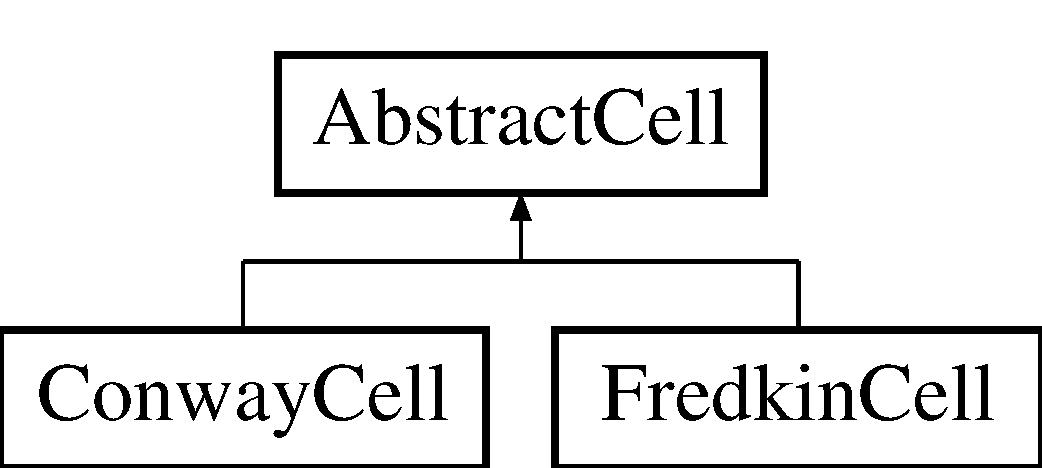
\includegraphics[height=2.000000cm]{classAbstractCell}
\end{center}
\end{figure}
\subsection*{Public Member Functions}
\begin{DoxyCompactItemize}
\item 
\hypertarget{classAbstractCell_a525a759bf4c2a9a70dec10d2569e1b93}{virtual int {\bfseries act} ()=0}\label{classAbstractCell_a525a759bf4c2a9a70dec10d2569e1b93}

\item 
\hypertarget{classAbstractCell_a6a54874737323dc8a67007e15ef35a40}{virtual void {\bfseries print\-\_\-cell} ()=0}\label{classAbstractCell_a6a54874737323dc8a67007e15ef35a40}

\item 
\hypertarget{classAbstractCell_ab9de226124a08d3f718c35785f92ed31}{virtual void {\bfseries living} (\hyperlink{structLocale}{Locale} l)=0}\label{classAbstractCell_ab9de226124a08d3f718c35785f92ed31}

\item 
\hypertarget{classAbstractCell_a7ff5f687d3245955dccc2653a872dc25}{virtual bool {\bfseries heterogeneous\-\_\-grid\-\_\-act} ()=0}\label{classAbstractCell_a7ff5f687d3245955dccc2653a872dc25}

\end{DoxyCompactItemize}
\subsection*{Public Attributes}
\begin{DoxyCompactItemize}
\item 
\hypertarget{classAbstractCell_ae61feab8faaed128353038f78e7072b2}{int {\bfseries living\-\_\-neighbors}}\label{classAbstractCell_ae61feab8faaed128353038f78e7072b2}

\item 
\hypertarget{classAbstractCell_aa92e42d5bb67f3249d8e2dde2c3228e7}{bool {\bfseries alive}}\label{classAbstractCell_aa92e42d5bb67f3249d8e2dde2c3228e7}

\end{DoxyCompactItemize}
\subsection*{Friends}
\begin{DoxyCompactItemize}
\item 
\hypertarget{classAbstractCell_a4ceaaf9d661d54f6ed2b18cf0d8830a6}{class {\bfseries Cell}}\label{classAbstractCell_a4ceaaf9d661d54f6ed2b18cf0d8830a6}

\end{DoxyCompactItemize}


The documentation for this class was generated from the following file\-:\begin{DoxyCompactItemize}
\item 
Life.\-h\end{DoxyCompactItemize}

\hypertarget{classCell}{\section{Cell Class Reference}
\label{classCell}\index{Cell@{Cell}}
}
\subsection*{Public Member Functions}
\begin{DoxyCompactItemize}
\item 
\hypertarget{classCell_a4f4c57dd913d6cb58287d4193eefa69f}{void {\bfseries living} (\hyperlink{structLocale}{Locale})}\label{classCell_a4f4c57dd913d6cb58287d4193eefa69f}

\item 
\hypertarget{classCell_a11a25348c84b39292c8f10923b3427d1}{{\bfseries Cell} (\hyperlink{classAbstractCell}{Abstract\-Cell} $\ast$=nullptr)}\label{classCell_a11a25348c84b39292c8f10923b3427d1}

\item 
\hypertarget{classCell_a1bfc6791f9916c0436d1f6242f6bb213}{int {\bfseries act} ()}\label{classCell_a1bfc6791f9916c0436d1f6242f6bb213}

\item 
\hypertarget{classCell_a532b26bf445ab573b1bc00b876c9ca42}{\hyperlink{classAbstractCell}{Abstract\-Cell} $\ast$ {\bfseries operator-\/$>$} ()}\label{classCell_a532b26bf445ab573b1bc00b876c9ca42}

\end{DoxyCompactItemize}
\subsection*{Public Attributes}
\begin{DoxyCompactItemize}
\item 
\hypertarget{classCell_a370fa2c4f2f8a06a5886a72f34ba492b}{\hyperlink{classAbstractCell}{Abstract\-Cell} $\ast$ {\bfseries abstractcell\-\_\-ptr}}\label{classCell_a370fa2c4f2f8a06a5886a72f34ba492b}

\end{DoxyCompactItemize}
\subsection*{Friends}
\begin{DoxyCompactItemize}
\item 
\hypertarget{classCell_af9ef66cb5aeb8b53ce639ba912ca5dbf}{class {\bfseries Fredkin\-Cell}}\label{classCell_af9ef66cb5aeb8b53ce639ba912ca5dbf}

\item 
\hypertarget{classCell_a3d40ad4ebe6b5876817523e88934a66b}{class {\bfseries Conway\-Cell}}\label{classCell_a3d40ad4ebe6b5876817523e88934a66b}

\end{DoxyCompactItemize}


The documentation for this class was generated from the following files\-:\begin{DoxyCompactItemize}
\item 
Life.\-h\item 
Life.\-c++\end{DoxyCompactItemize}

\hypertarget{classConwayCell}{\section{Conway\-Cell Class Reference}
\label{classConwayCell}\index{Conway\-Cell@{Conway\-Cell}}
}
Inheritance diagram for Conway\-Cell\-:\begin{figure}[H]
\begin{center}
\leavevmode
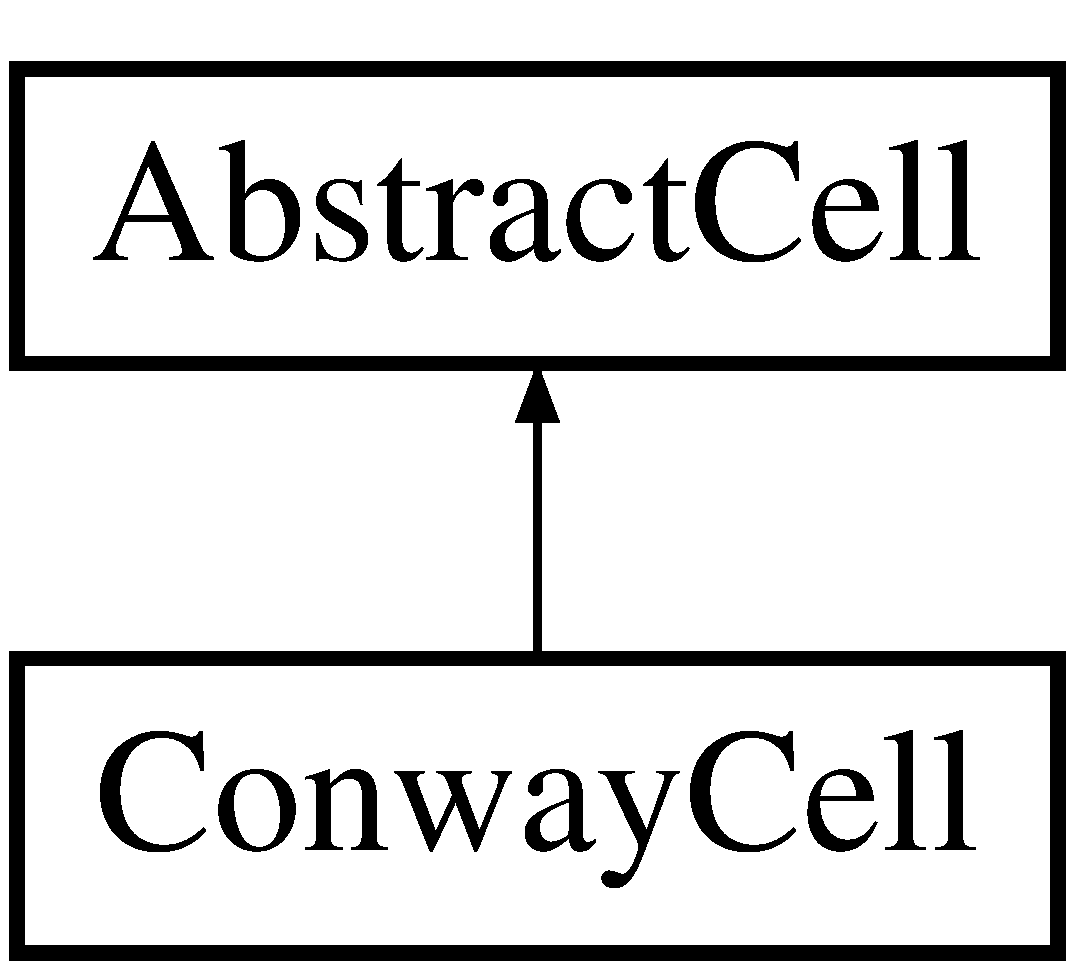
\includegraphics[height=2.000000cm]{classConwayCell}
\end{center}
\end{figure}
\subsection*{Public Member Functions}
\begin{DoxyCompactItemize}
\item 
\hypertarget{classConwayCell_a29d644f02614791cc1599bcb452ff640}{{\bfseries Conway\-Cell} (bool living=false)}\label{classConwayCell_a29d644f02614791cc1599bcb452ff640}

\item 
\hypertarget{classConwayCell_a1805b09ec0ce84f68e986d592185309f}{int {\bfseries act} ()}\label{classConwayCell_a1805b09ec0ce84f68e986d592185309f}

\item 
\hypertarget{classConwayCell_a031aefa5a4a75cc0fc64ee4b8907d2f0}{void {\bfseries living} (\hyperlink{structLocale}{Locale})}\label{classConwayCell_a031aefa5a4a75cc0fc64ee4b8907d2f0}

\item 
\hypertarget{classConwayCell_aa93e8d9d3a1c6ec2eeb7586c3e082a89}{void {\bfseries print\-\_\-cell} ()}\label{classConwayCell_aa93e8d9d3a1c6ec2eeb7586c3e082a89}

\item 
\hypertarget{classConwayCell_aca833d0cfa7e1d361700302ec3e81f5d}{bool {\bfseries heterogeneous\-\_\-grid\-\_\-act} ()}\label{classConwayCell_aca833d0cfa7e1d361700302ec3e81f5d}

\item 
\hypertarget{classConwayCell_a6c7be773417cf17223228fa676765e17}{\hyperlink{classConwayCell}{Conway\-Cell} $\ast$ {\bfseries operator-\/$>$} ()}\label{classConwayCell_a6c7be773417cf17223228fa676765e17}

\end{DoxyCompactItemize}
\subsection*{Additional Inherited Members}


The documentation for this class was generated from the following files\-:\begin{DoxyCompactItemize}
\item 
Life.\-h\item 
Life.\-c++\end{DoxyCompactItemize}

\hypertarget{classFredkinCell}{\section{Fredkin\-Cell Class Reference}
\label{classFredkinCell}\index{Fredkin\-Cell@{Fredkin\-Cell}}
}
Inheritance diagram for Fredkin\-Cell\-:\begin{figure}[H]
\begin{center}
\leavevmode
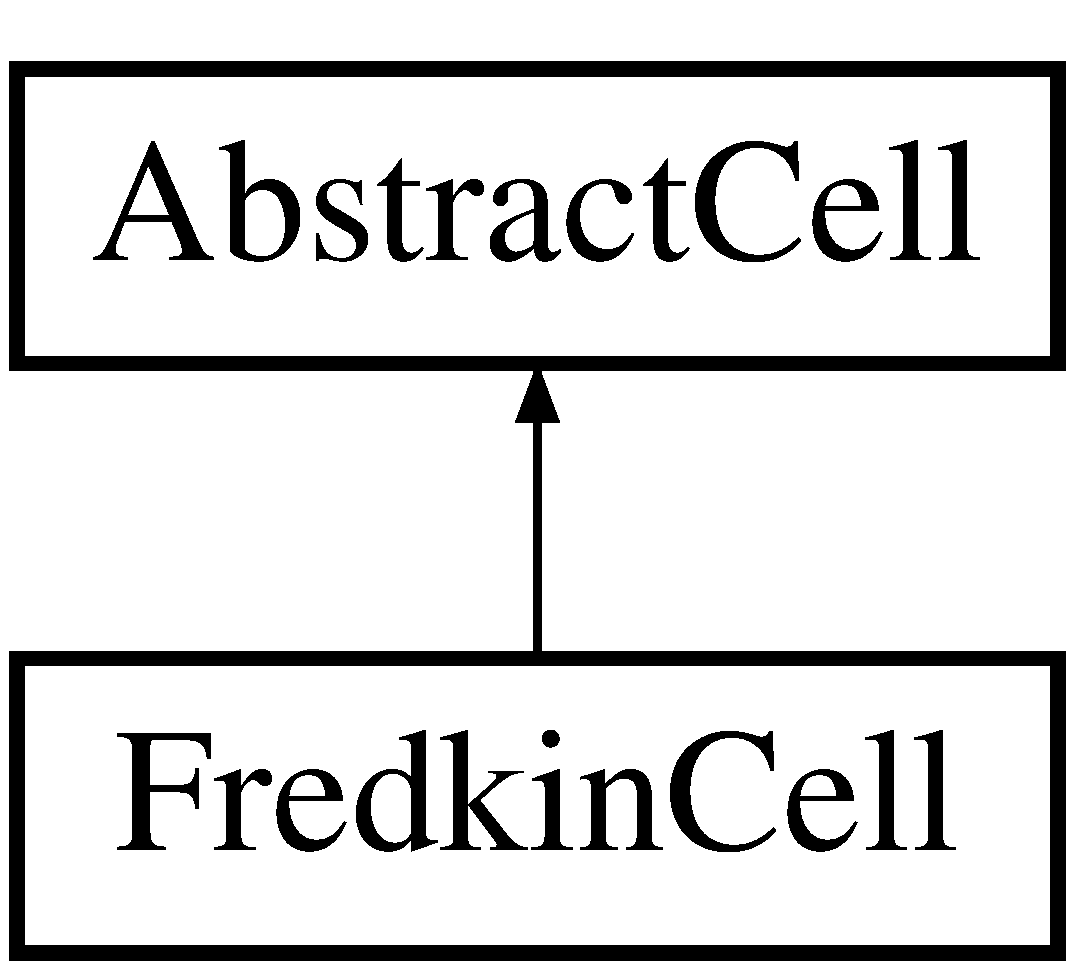
\includegraphics[height=2.000000cm]{classFredkinCell}
\end{center}
\end{figure}
\subsection*{Public Member Functions}
\begin{DoxyCompactItemize}
\item 
\hypertarget{classFredkinCell_a10a38c451ddc914d833969289cbd7b07}{{\bfseries Fredkin\-Cell} (bool living=false)}\label{classFredkinCell_a10a38c451ddc914d833969289cbd7b07}

\item 
\hypertarget{classFredkinCell_a06443820d9015c235297bff1c7275562}{int {\bfseries act} ()}\label{classFredkinCell_a06443820d9015c235297bff1c7275562}

\item 
\hypertarget{classFredkinCell_aaea67599210c77e6a57695aa8cb3c15a}{void {\bfseries print\-\_\-cell} ()}\label{classFredkinCell_aaea67599210c77e6a57695aa8cb3c15a}

\item 
\hypertarget{classFredkinCell_ac99c9fe832682b2bb95a19c44c84bfb6}{void {\bfseries living} (\hyperlink{structLocale}{Locale})}\label{classFredkinCell_ac99c9fe832682b2bb95a19c44c84bfb6}

\item 
\hypertarget{classFredkinCell_a1249a32202e5b1b5188f25087a082ac6}{bool {\bfseries heterogeneous\-\_\-grid\-\_\-act} ()}\label{classFredkinCell_a1249a32202e5b1b5188f25087a082ac6}

\item 
\hypertarget{classFredkinCell_a743df8596f94d55aceeb96d35377d67b}{\hyperlink{classFredkinCell}{Fredkin\-Cell} $\ast$ {\bfseries operator-\/$>$} ()}\label{classFredkinCell_a743df8596f94d55aceeb96d35377d67b}

\end{DoxyCompactItemize}
\subsection*{Public Attributes}
\begin{DoxyCompactItemize}
\item 
\hypertarget{classFredkinCell_a755dea54626a9742e4dad6a03755706b}{int {\bfseries age}}\label{classFredkinCell_a755dea54626a9742e4dad6a03755706b}

\end{DoxyCompactItemize}


The documentation for this class was generated from the following files\-:\begin{DoxyCompactItemize}
\item 
Life.\-h\item 
Life.\-c++\end{DoxyCompactItemize}

\hypertarget{classLife}{\section{Life$<$ Cell\-Type $>$ Class Template Reference}
\label{classLife}\index{Life$<$ Cell\-Type $>$@{Life$<$ Cell\-Type $>$}}
}
\subsection*{Public Member Functions}
\begin{DoxyCompactItemize}
\item 
\hypertarget{classLife_a04473ab6c263b204c9b8a862085a4200}{{\bfseries Life} (int rows, int cols, istream \&is=cin)}\label{classLife_a04473ab6c263b204c9b8a862085a4200}

\item 
\hypertarget{classLife_a3cf922d10c62e7cb828858055c19ed3e}{void {\bfseries populate\-\_\-heterogeneous\-\_\-grid} ()}\label{classLife_a3cf922d10c62e7cb828858055c19ed3e}

\item 
\hypertarget{classLife_a7643f257a1f163f466fede4298905d19}{void {\bfseries populate\-\_\-homogeneous\-\_\-grid} ()}\label{classLife_a7643f257a1f163f466fede4298905d19}

\item 
\hypertarget{classLife_ad442b2e0d970e8a9d61548a7a456f6c3}{Cell\-Type \& {\bfseries at} (int rows, int cols)}\label{classLife_ad442b2e0d970e8a9d61548a7a456f6c3}

\item 
\hypertarget{classLife_af4898790bfc58aeafb14f4f52af5e781}{Cell\-Type \& {\bfseries at} (int n)}\label{classLife_af4898790bfc58aeafb14f4f52af5e781}

\item 
\hypertarget{classLife_ac30078b08598a338b254d37672b050ae}{\hyperlink{classLife__Iterator}{Life\-\_\-\-Iterator}$<$ Cell\-Type $>$ {\bfseries begin} ()}\label{classLife_ac30078b08598a338b254d37672b050ae}

\item 
\hypertarget{classLife_a9ac3ffc992bbd32addc10354c8acae87}{\hyperlink{classLife__Iterator}{Life\-\_\-\-Iterator}$<$ Cell\-Type $>$ {\bfseries end} ()}\label{classLife_a9ac3ffc992bbd32addc10354c8acae87}

\item 
\hypertarget{classLife_a6fd0fa4a0dd7f0ef932fc187b3e11eb4}{int {\bfseries convert} (int rows, int cols)}\label{classLife_a6fd0fa4a0dd7f0ef932fc187b3e11eb4}

\item 
\hypertarget{classLife_ad94ec4c8e59c2defd69cb812bf3f1b95}{pair$<$ int, int $>$ {\bfseries convert} (int i)}\label{classLife_ad94ec4c8e59c2defd69cb812bf3f1b95}

\item 
\hypertarget{classLife_a747a109435a599db7dbcef99cc83d42c}{void {\bfseries print\-\_\-grid} ()}\label{classLife_a747a109435a599db7dbcef99cc83d42c}

\item 
\hypertarget{classLife_a34cdf0c8bec9334a20c9eafadc967a52}{void {\bfseries step} ()}\label{classLife_a34cdf0c8bec9334a20c9eafadc967a52}

\item 
\hypertarget{classLife_a05eee381f80732bee4e16d1fe0863dac}{void {\bfseries set\-\_\-living} ()}\label{classLife_a05eee381f80732bee4e16d1fe0863dac}

\item 
\hypertarget{classLife_aedd5f65664d05a8dbfaa012eb9c5d4ab}{void {\bfseries process\-\_\-cells} ()}\label{classLife_aedd5f65664d05a8dbfaa012eb9c5d4ab}

\item 
\hypertarget{classLife_aa9adce7420176d9b06437acbcedc4cdf}{void {\bfseries evolve} ()}\label{classLife_aa9adce7420176d9b06437acbcedc4cdf}

\item 
\hypertarget{classLife_a7eb3bd1c61d0c047b1c74f1d22367094}{{\bfseries F\-R\-I\-E\-N\-D\-\_\-\-T\-E\-S\-T} (Life\-Fixture, Life\-\_\-\-Constructor\-\_\-1)}\label{classLife_a7eb3bd1c61d0c047b1c74f1d22367094}

\end{DoxyCompactItemize}
\subsection*{Public Attributes}
\begin{DoxyCompactItemize}
\item 
\hypertarget{classLife_a5e249348368f58125728bf6f1888ab0c}{int {\bfseries grid\-\_\-rows}}\label{classLife_a5e249348368f58125728bf6f1888ab0c}

\item 
\hypertarget{classLife_aaf218714ee6df928b2273350a499136c}{int {\bfseries grid\-\_\-cols}}\label{classLife_aaf218714ee6df928b2273350a499136c}

\item 
\hypertarget{classLife_a2d286b3c1129abc0587a0b85391e1fb3}{int {\bfseries evolutions}}\label{classLife_a2d286b3c1129abc0587a0b85391e1fb3}

\item 
\hypertarget{classLife_a84708bb3de8658b0aa2d2749b7017c66}{int {\bfseries frequency}}\label{classLife_a84708bb3de8658b0aa2d2749b7017c66}

\item 
\hypertarget{classLife_a43ab920e05039c94378ddee6f54b85e9}{int {\bfseries generation}}\label{classLife_a43ab920e05039c94378ddee6f54b85e9}

\item 
\hypertarget{classLife_a58260f9a901a41f1318b9a1dac4f66fe}{int {\bfseries population}}\label{classLife_a58260f9a901a41f1318b9a1dac4f66fe}

\item 
\hypertarget{classLife_a830fc290bc14345376fb66649968e111}{vector$<$ Cell\-Type $>$ {\bfseries grid}}\label{classLife_a830fc290bc14345376fb66649968e111}

\item 
\hypertarget{classLife_a9844b0b9fcb2405b9d8914a954e87d61}{istream \& {\bfseries input\-\_\-stream}}\label{classLife_a9844b0b9fcb2405b9d8914a954e87d61}

\item 
\hypertarget{classLife_a82ac9f74b82e51e6a31ea25b5110c863}{bool {\bfseries is\-\_\-hetero}}\label{classLife_a82ac9f74b82e51e6a31ea25b5110c863}

\end{DoxyCompactItemize}


The documentation for this class was generated from the following file\-:\begin{DoxyCompactItemize}
\item 
Life.\-h\end{DoxyCompactItemize}

\hypertarget{classLife__Iterator}{\section{Life\-\_\-\-Iterator$<$ Cell\-Type $>$ Class Template Reference}
\label{classLife__Iterator}\index{Life\-\_\-\-Iterator$<$ Cell\-Type $>$@{Life\-\_\-\-Iterator$<$ Cell\-Type $>$}}
}
Inheritance diagram for Life\-\_\-\-Iterator$<$ Cell\-Type $>$\-:\begin{figure}[H]
\begin{center}
\leavevmode
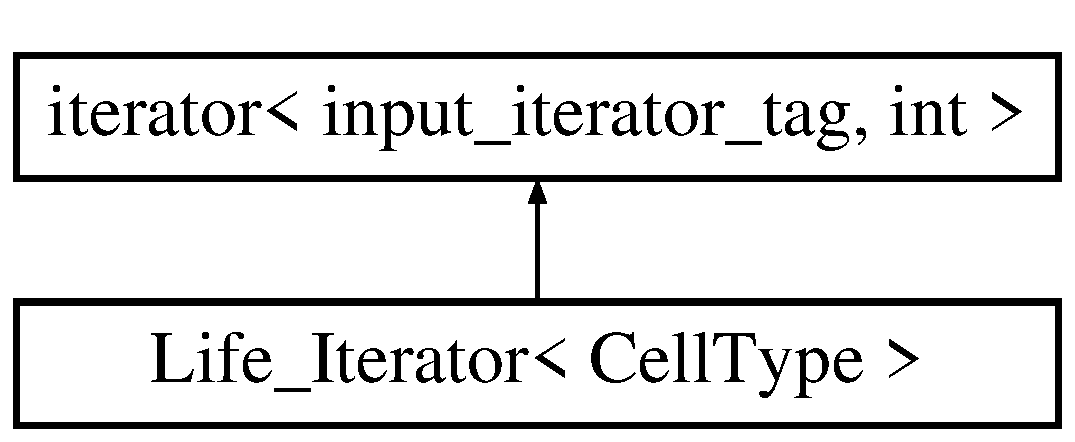
\includegraphics[height=2.000000cm]{classLife__Iterator}
\end{center}
\end{figure}
\subsection*{Public Member Functions}
\begin{DoxyCompactItemize}
\item 
\hypertarget{classLife__Iterator_a1cc454590f21bf60efa60008600e220e}{{\bfseries Life\-\_\-\-Iterator} (int v, \hyperlink{classLife}{Life}$<$ Cell\-Type $>$ $\ast$li)}\label{classLife__Iterator_a1cc454590f21bf60efa60008600e220e}

\item 
\hypertarget{classLife__Iterator_a96a44af672e18c95afdb49bfc8116273}{bool {\bfseries operator==} (const \hyperlink{classLife__Iterator}{Life\-\_\-\-Iterator} \&rhs) const }\label{classLife__Iterator_a96a44af672e18c95afdb49bfc8116273}

\item 
\hypertarget{classLife__Iterator_a3fae7afeb06ecdf6d2e6779a926c5b1a}{bool {\bfseries operator!=} (const \hyperlink{classLife__Iterator}{Life\-\_\-\-Iterator} \&rhs) const }\label{classLife__Iterator_a3fae7afeb06ecdf6d2e6779a926c5b1a}

\item 
\hypertarget{classLife__Iterator_a25f911f90ba7d3cf0f3190e33f5149e4}{const Cell\-Type \& {\bfseries operator$\ast$} () const }\label{classLife__Iterator_a25f911f90ba7d3cf0f3190e33f5149e4}

\item 
\hypertarget{classLife__Iterator_a24ab346197518ae395e7d55a106bc43c}{\hyperlink{classLife__Iterator}{Life\-\_\-\-Iterator} \& {\bfseries operator++} ()}\label{classLife__Iterator_a24ab346197518ae395e7d55a106bc43c}

\item 
\hypertarget{classLife__Iterator_a5dda74f118e048f7c263a19ee57dd4a7}{\hyperlink{classLife__Iterator}{Life\-\_\-\-Iterator} {\bfseries operator++} (int)}\label{classLife__Iterator_a5dda74f118e048f7c263a19ee57dd4a7}

\end{DoxyCompactItemize}
\subsection*{Public Attributes}
\begin{DoxyCompactItemize}
\item 
\hypertarget{classLife__Iterator_a78be6d8aa88e150bcec6b2d37ce477fe}{int {\bfseries \-\_\-p}}\label{classLife__Iterator_a78be6d8aa88e150bcec6b2d37ce477fe}

\item 
\hypertarget{classLife__Iterator_adcfcecd7ab3886cda6b1389691ad0b1b}{\hyperlink{classLife}{Life}$<$ Cell\-Type $>$ $\ast$ {\bfseries d}}\label{classLife__Iterator_adcfcecd7ab3886cda6b1389691ad0b1b}

\end{DoxyCompactItemize}


The documentation for this class was generated from the following file\-:\begin{DoxyCompactItemize}
\item 
Life.\-h\end{DoxyCompactItemize}

\hypertarget{structLocale}{\section{Locale Struct Reference}
\label{structLocale}\index{Locale@{Locale}}
}
\subsection*{Public Attributes}
\begin{DoxyCompactItemize}
\item 
\hypertarget{structLocale_ac655747bc826e31f01e8e5acfb5f6268}{int {\bfseries n}}\label{structLocale_ac655747bc826e31f01e8e5acfb5f6268}

\item 
\hypertarget{structLocale_a37af295258b1421ae8e0a865462153bf}{int {\bfseries ne}}\label{structLocale_a37af295258b1421ae8e0a865462153bf}

\item 
\hypertarget{structLocale_a9568285f2119b9ce5dff2505f35b064f}{int {\bfseries e}}\label{structLocale_a9568285f2119b9ce5dff2505f35b064f}

\item 
\hypertarget{structLocale_a1bd7acefe62da8a46718881544f85d26}{int {\bfseries se}}\label{structLocale_a1bd7acefe62da8a46718881544f85d26}

\item 
\hypertarget{structLocale_a06131abdca4f375798ec1114a966bd28}{int {\bfseries s}}\label{structLocale_a06131abdca4f375798ec1114a966bd28}

\item 
\hypertarget{structLocale_a41d08cd7df25b24230eadc9e82b15f62}{int {\bfseries sw}}\label{structLocale_a41d08cd7df25b24230eadc9e82b15f62}

\item 
\hypertarget{structLocale_ac592efb1d5356f2f180fb8cb9b8eeee4}{int {\bfseries w}}\label{structLocale_ac592efb1d5356f2f180fb8cb9b8eeee4}

\item 
\hypertarget{structLocale_a2ab054e7597d801de5821c56ce4baf9e}{int {\bfseries nw}}\label{structLocale_a2ab054e7597d801de5821c56ce4baf9e}

\end{DoxyCompactItemize}


The documentation for this struct was generated from the following file\-:\begin{DoxyCompactItemize}
\item 
Life.\-h\end{DoxyCompactItemize}

%--- End generated contents ---

% Index
\newpage
\phantomsection
\addcontentsline{toc}{chapter}{Index}
\printindex

\end{document}
